\documentclass{../../kalkulus-ppt}



\author[Tetew]{Teosofi Hidayah Agung}
\date{19 September 2024}
\title[Kalkulus 1 - Bab 3]{Limit dan Kekontinuan}
\institute[Matematika ITS]{Departemen Matematika\\ Institut Teknologi Sepuluh Nopember}
\titlegraphic{{\includegraphics[scale=0.3]{ITS.png}$\quad$\includegraphics[scale=0.02]{M.png}}}

\newcommand{\dom}{\mathcal{D}}
\newcommand{\rng}{\mathcal{R}}

\renewcommand{\arraystretch}{1.5}

\begin{document}
{\usebackgroundtemplate{
    \tikz[overlay,remember picture] \node[opacity=0.09, at=(current page.center)]{\includegraphics[width=\paperwidth]{limitless}};}
\begin{frame}
    \titlepage
\end{frame}
}

\AtBeginSection{
    {
            \begin{frame}{Daftar isi}
                \tableofcontents[currentsection]
                % \begin{tikzpicture}[overlay, remember picture] 
                %     \node at ([yshift=.5cm]current page.south east) [
                %         anchor = south east, 
                %         ] {
                %     \animategraphics[autoplay,loop,width=0.2\textwidth]{30}{Arisu Dance/Arisu Dance-}{0}{186}
                %     };
                % \end{tikzpicture}
            \end{frame}}
}

\section{Notasi Limit}
\begin{frame}
    \frametitle{\insertsection}
    \begin{definisi}
        Notasi limit yang biasanya dibaca ``limit $f(x)$ saat $x$ \textbf{mendekati} $a$ adalah $L$'' dituliskan sebagai
        \[\lim_{x\to a} f(x)=L,\]
        Artinya jika kita mengambil nilai $x$ yang sangat dekat dengan $a$, maka $f(x)$ akan sangat dekat dengan $L$.
    \end{definisi}
    \onslide<2->{
        \setbeamercolor{item}{fg=PastelGreen!50!HIMAmuda}
        \begin{alertblock}{Catatan}
            \begin{itemize}
                \item Kata ``mendekati'' jangan disamakan dengan ``menuju''.
                \item Nilai $f(a)$ tidak harus sama dengan $L$ atau bahkan $f(a)$ tidak terdefinisi.
                \item Nilai $f(x)$ untuk $x=a$ tidak mempengaruhi nilai limit.
            \end{itemize}
        \end{alertblock}}
\end{frame}

\begin{frame}
    \frametitle{\insertsection}
    \begin{figure}[h!]
        \centering
        \begin{tikzpicture}[scale=.4,cap=round]
            \tikzset{axes/.style={}}
            % The graphic

            \begin{scope}[style=axes]
                \draw[->] (-7.5,0) -- (7.5,0) node[right] {$x$};
                \draw[->] (0,-7.5)-- (0,7.5) node[above] {$y$};
                \foreach \x/\xtext in {-6/-12,  -4/-8,  -2/-4,     2/4,  4/8, 6/12}
                    {\ifnum\x=2
                        \else
                            \draw[xshift=\x cm] (0pt,2.6pt) -- (0pt,-2.6pt) node[below,font=\scriptsize]
                            {$\xtext$};
                        \fi
                    }
                \foreach \y/\ytext in {-6/-12,  -4/-8,  -2/-4,    2/4,  4/8,  6.5/13}
                \draw[yshift=\y cm] (2.6pt,0pt) -- (-2.6pt,0pt) node[left,font=\scriptsize]
                {$\ytext$};
                \draw[domain=-4.1:2.9,smooth,variable=\x,brown,thick] plot ({\x},{.5*(3+4*\x)});
                \node at (-6,-3) [brown] {\scriptsize$\displaystyle f(x)=\frac{2x^2-5x-12}{x-4}$};
                \draw[dashed] (2.5,0)--(2.5,6.5)--(0,6.5);
                \draw[dashed] (1.5,0)--(1.5,4.5)--(0,4.5);
            \end{scope}
            \draw[cyan,thick] (0,5.5) -- (-1,5.5) node[left,font=\scriptsize](11){11};
            \node[single arrow,cyan,minimum height=1.5cm,rotate=-90,fill,transform
                shape,anchor=east,opacity=0.3] at(11.north){};
            \node[single arrow,cyan,minimum height=1.5cm,rotate=90,fill,transform
                shape,anchor=east,opacity=0.3] at(11.south){};
            \draw[red,thick,dashed] (2,0) -- (2,5.5);
            \draw[blue,thick,dashed] (0,5.5) -- (2,5.5);
            \node[text=red,font=\scriptsize] (4) at (2,-0.5) {4};
            \node[single arrow,red,minimum height=1.5cm,rotate=0,fill,transform
                shape,anchor=east,opacity=0.3] at(4.west){};
            \node[single arrow,red,minimum height=1.5cm,rotate=180,fill,transform
                shape,anchor=east,opacity=0.3] at(4.east){};
            %
            \matrix[matrix of math nodes,nodes={font=\scriptsize,text width=11mm,align=right,inner sep=3pt,
                    text height=1.5ex,text depth=.25ex,draw=gray!40,ultra thin},draw,inner
            sep=0pt,ampersand replacement=\&] (mat)
            at (16,-0.5){
            |[fill=green!40!gray,align=left]| x      \& |[fill=green!40!gray,align=left]|f(x)    \\
            3.9    \& 10.8    \\
            3.99   \& 10.98   \\
            3.999  \& 10.998  \\
            |[text=red!90,align=center]|\vdots \& |[text=cyan!90,align=center]|\vdots  \\
            |[text=red!90,align=center]| 4 \& |[text=cyan!90,align=center]| 11 \\
            |[text=red!90,align=center]|\vdots \& |[text=cyan!90,align=center]|\vdots  \\
            4.001  \& 11.002  \\
            4.01   \& 11.02   \\
            4.1    \& 11.2    \\
            };
            \draw[thin,gray!40] (mat.north west) -- (mat.north east);
            \draw[line width=1mm,-latex,red!90] ([xshift=-4mm,yshift=-3mm]mat-2-1.north west)
            node[xshift=-5mm,anchor=east,align=left,font=\tiny,rotate=90]{Nilai input\\
                mendekati 4 dari kiri.}
            --([xshift=-4mm,yshift=-8mm]mat-5-1.west);
            \draw[line width=1mm,latex-,red!90] ([xshift=-4mm,yshift=2mm]mat-6-1.south west)
            node[xshift=-5mm,anchor=east,align=left,font=\tiny,rotate=90]{Nilai input\\
                mendekati 4 dari kanan.}
            --  ([xshift=-4mm,yshift=-4mm]mat-10-1.west);
            \draw[line width=1mm,-latex,cyan!90] ([xshift=4mm,yshift=-3mm]mat-2-2.north east)
            node[xshift=5mm,anchor=west,align=left,font=\tiny,rotate=-90]{Nilai output\\
                mendekati 11 dari kiri.}
            --([xshift=4mm,yshift=-8mm]mat-5-2.east);
            \draw[line width=1mm,latex-,cyan!90] ([xshift=4mm,yshift=2mm]mat-6-2.south east)
            node[xshift=5mm,anchor=west,align=left,font=\tiny,rotate=-90]{Nilai output\\
                mendekati 11 dari kanan.}
            --  ([xshift=4mm,yshift=2mm]mat-10-2.south east);
            \draw[black,fill=white] (2,5.5) circle (4pt);
        \end{tikzpicture}
        \caption{Limit secara numerik}
    \end{figure}
\end{frame}

\begin{frame}
    \frametitle{\insertsection}
    Dalam kasus $f(x)=\frac{|x|}{x}$, fungsi ini tidak memiliki limit saat $x$ mendekati 0. Mengapa?
    \begin{figure}[h!]
        \centering
        \begin{tikzpicture}[scale=0.8]
            \draw [->] (-3,0) -- (3,0) node [right] {\footnotesize$x$};
            \draw [->] (0,-3) -- (0,3) node [above] {\footnotesize$y$};

            \draw [domain=-2.9:0, samples=50, thick, blue] plot (\x, {-1});
            \draw [domain=0:2.9, samples=50, thick, blue] plot (\x, {1});

            \draw [domain=-3:3, samples=10, darkgray, dashed] plot (0, {\x});

            \draw[fill=white] (0,-1) circle (0.1);
            \draw[fill=white] (0,1) circle (0.1);

            \node [below] at (-2,0) {\footnotesize$-2$};
            \node [below] at (2,0) {\footnotesize$2$};
            \node [below left] at (0,-1) {\footnotesize$-1$};
            \node [above left] at (0,1) {\footnotesize$1$};

            \node at (7,0) {\footnotesize$f(x)=\begin{cases}
                        -1, & x<0 \\
                        1,  & x>0
                    \end{cases}$};
        \end{tikzpicture}
    \end{figure}
    \onslide<2->{Fungsi $f(x)=\frac{|x|}{x}$ tidak memiliki limit saat $x$ mendekati 0 karena nilai limit dari kiri ($-1$) tidak sama dengan nilai limit dari kanan ($1$).}
\end{frame}

\section{Perhitungan Limit}
\begin{frame}
    \frametitle{\insertsection}
    \begin{teorema}
        Misalkan $f$ dan $g$ adalah dua fungsi dengan $\displaystyle\lim_{x\to a} f(x)=L$ dan $\displaystyle\lim_{x\to a} g(x)=M$, maka
        \begin{enumerate}
            \item $\displaystyle\lim_{x\to a} [f(x)+g(x)]=L+M$
            \item $\displaystyle\lim_{x\to a} [f(x)-g(x)]=L-M$
            \item $\displaystyle\lim_{x\to a} [f(x)\cdot g(x)]=L\cdot M$
            \item Jika $M\ne 0$, maka $\displaystyle\lim_{x\to a} \frac{f(x)}{g(x)}=\frac{L}{M}$
            \item $\displaystyle\lim_{x\to a} \sqrt[n]{f(x)}=\sqrt[n]{L}$, dengan $n$ bilangan bulat positif
        \end{enumerate}
    \end{teorema}
\end{frame}
\begin{frame}
    \frametitle{\insertsection}
    \begin{contoh}
        \begin{itemize}
            \item $\displaystyle\lim_{x\to 2} x=2$
            \item $\displaystyle\lim_{x\to \frac{1}{2}} \frac{6x^2-x-1}{2x-1}=\frac{5}{2}$
            \item $\displaystyle\lim_{x\to 3} \frac{\sqrt{12-x}-3}{x-3}=-\frac{1}{6}$
            \item $\displaystyle\lim_{x\to 0} \frac{\sin x}{x}=1$
        \end{itemize}
    \end{contoh}
\end{frame}
\begin{frame}
    \frametitle{\insertsection}
    \begin{definisi}
        Domain fungsi $f$ adalah himpunan semua nilai $x$ yang memenuhi $f(x)$ didefinisikan. Notasi domain fungsi $f$ adalah \[\dom(f)=\{x\in\R\mid f(x)\text{ terdefinisi}\}\]
        Range fungsi $f$ adalah himpunan semua nilai $f(x)$ yang mungkin diperoleh saat $x$ berjalan di domain fungsi $f$. Notasi range fungsi $f$ adalah \[\rng(f)=\{f(x)\mid x\in\dom(f)\}\]
    \end{definisi}
\end{frame}

\begin{frame}
    \frametitle{\insertsection}
    \begin{table}
        \centering
        \begin{tabular}{|c|c|c|c|c|}
            \hline
            \rowcolor{HIMAmuda}
                                                & \multicolumn{2}{c|}{\textbf{Domain}} & \multicolumn{2}{c|}{\textbf{Range}}                                                           \\
            \cline{2-5}
            \rowcolor{HIMAmuda}
            \multirow{-2}{*}{\textbf{Fungsi}}   & \textbf{Himpunan}                    & \textbf{Interval}                   & \textbf{Himpunan}         & \textbf{Interval}           \\
            \hline
            $f(x)=ax+b$                         & $\R$                                 & $(-\infty,\infty)$                  & $\R$                      & $(-\infty,\infty)$          \\
            $f(x)=a(x-p)^2+q$                   & $\R$                                 & $(-\infty,\infty)$                  & $\{f(x)\mid f(x)\geq q\}$ & $[q,\infty)$                \\
            $\displaystyle f(x)=\frac{1}{g(x)}$ & $\{x\mid g(x)\ne 0\}$                & $(-\infty,\infty)$                  & $\{f(x)\mid f(x)\ne 0\}$  & $(-\infty,0)\cup(0,\infty)$ \\
            $f(x)=\sqrt{g(x)}$                  & $\{x\mid g(x)\geq 0\}$               & $[0,\infty)$                        & $\{f(x)\mid f(x)\geq 0\}$ & $[0,\infty)$                \\
            \hline
        \end{tabular}
        \caption{Domain dan Range beberapa fungsi}
    \end{table}
\end{frame}

\begin{frame}
    \frametitle{\insertsection}
    \begin{exampleblock}{Latihan}
        \begin{enumerate}
            \item Jika $f(t)=\begin{cases}
                          2t+1,  & t\geq 0 \\
                          t^2-1, & t<0
                      \end{cases}$, tentukan $f(x^2)$
            \item Tulislah dalam fungsi sepotong-sepotong $f(x)=|4+|x-1||$
            \item Tentukan domain dan range dari fungsi $\displaystyle f(x)=\frac{1}{\sqrt{4-x^2}}$
        \end{enumerate}
    \end{exampleblock}
\end{frame}

\section{Limit di Tak-Hingga}
\begin{frame}
    \frametitle{\insertsection}
    \begin{definisi}
        Misalkan $f$ dan $g$ adalah dua fungsi. Operasi-operasi pada fungsi adalah sebagai berikut
        \begin{enumerate}
            \item Penjumlahan: $(f+g)(x)=f(x)+g(x)$
            \item Pengurangan: $(f-g)(x)=f(x)-g(x)$
            \item Perkalian: $(f\cdot g)(x)=f(x)\cdot g(x)$
            \item Pembagian: $\left(\displaystyle\frac{f}{g}\right)(x)=\displaystyle\frac{f(x)}{g(x)}$
        \end{enumerate}
        Kemudian untuk domain dari fungsi hasil operasi adalah \[\dom(f\pm g)=\dom(f\cdot g)=\dom(f)\cap\dom(g)\]
        Sedangkan untuk kasus pembagian harus memenuhi $g(x)\ne 0$, sehingga
        \[\dom\left(f/g\right)=(\dom(f)\cap\dom(g)) - \{x\mid g(x)=0\}\]
    \end{definisi}
\end{frame}

\begin{frame}
    \frametitle{\insertsection}
    \begin{definisi}
        Komposisi fungsi $f$ dan $g$ adalah fungsi baru yang didefinisikan sebagai
        \[(f\circ g)(x)=f(g(x))\]
        Domain dari fungsi komposisi adalah
        \[\dom(f\circ g)=\{x\in\dom(g)\mid g(x)\in\dom(f)\}\]
    \end{definisi}
\end{frame}

\begin{frame}
    \frametitle{\insertsection}
    \begin{exampleblock}{Latihan}
        \begin{enumerate}
            \item Domain dari fungsi $\displaystyle f(x)=\frac{1}{x}+\sqrt{4-x^2}$ adalah
            \item Jika $f(g(x))=x^2+1$ dan $f(x)=\sqrt{x-1}$, tentukan $g(x)$
            \item Tentukan domain dari $g\circ f$ jika $f(x)=\sqrt{x^2-9}$ dan $\displaystyle g(x)=\frac{2}{x-3}$
        \end{enumerate}
    \end{exampleblock}
\end{frame}

\section{Kekontinuan}
\begin{frame}
    \frametitle{\insertsection}
    \begin{definisi}
        Grafik fungsi $f$ adalah himpunan semua titik $(x,y)$ dalam koordinat kartesius yang memenuhi persamaan $y=f(x)$.
    \end{definisi}
    \onslide<2->{\begin{teorema}
            Misalkan $y=f(x)$ adalah fungsi real, maka grafik $f(-x)$ adalah refleksi terhadap sumbu $y$ dari grafik $f(x)$ dan grafik $-f(x)$ adalah refleksi terhadap sumbu $x$ dari grafik $f(x)$.
        \end{teorema}}
\end{frame}

\begin{frame}
    \frametitle{\insertsection}
    Kasus $f(x)\implies f(-x)$
    \begin{figure}
        \begin{minipage}[b]{0.45\textwidth}
            \centering
            \begin{tikzpicture}[scale=0.8]
                \draw [->] (-2,0) -- (3,0) node [right] {\footnotesize$x$};
                \draw [->] (0,-1) -- (0,3) node [above] {\footnotesize$y$};

                \draw [domain=-1:3, samples=50, thick, blue] plot (\x, {sqrt(\x+1)});
                \node [below] at (-1,0) {\footnotesize$-1$};
            \end{tikzpicture}
            \caption*{$\boxed{y=\sqrt{x+1}}$}
        \end{minipage}
        \onslide<2->{\begin{minipage}[b]{0.45\textwidth}
                \centering
                \begin{tikzpicture}[scale=0.8]
                    \draw [->] (-3,0) -- (2,0) node [right] {\footnotesize$x$};
                    \draw [->] (0,-1) -- (0,3) node [above] {\footnotesize$y$};

                    \draw [domain=-1:2, samples=50, thick, cyan, dashed] plot (\x, {sqrt(\x+1)});
                    \draw [domain=-3:1, samples=50, thick, blue] plot (\x, {sqrt(-\x+1)});
                    \node [below] at (-1,0) {\footnotesize$-1$};
                    \node [below] at (1,0) {\footnotesize$1$};
                \end{tikzpicture}
                \caption*{$\boxed{y=\sqrt{-x+1}}$}
            \end{minipage}}
    \end{figure}
\end{frame}

\begin{frame}
    \frametitle{\insertsection}
    Kasus $f(x)\implies -f(x)$
    \begin{figure}
        \begin{minipage}[b]{0.45\textwidth}
            \centering
            \begin{tikzpicture}[scale=0.8]
                \draw [->] (-2,0) -- (4,0) node [right] {\footnotesize$x$};
                \draw [->] (0,-3) -- (0,3) node [above] {\footnotesize$y$};

                \draw [domain=1.35:4, samples=50, thick, blue] plot (\x, {1/(\x-1)});
                \draw [domain=-2:0.65, samples=50, thick, blue] plot (\x, {1/(\x-1)});
                \draw [domain=-3:3, samples=10, darkgray, dashed] plot (1, {\x});

                \node [below right] at (1,0) {\footnotesize$1$};
            \end{tikzpicture}
            \caption*{$\boxed{y=\frac{1}{x-1}}$}
        \end{minipage}
        \onslide<2->{\begin{minipage}[b]{0.45\textwidth}
                \centering
                \begin{tikzpicture}[scale=0.8]
                    \draw [->] (-2,0) -- (4,0) node [right] {\footnotesize$x$};
                    \draw [->] (0,-3) -- (0,3) node [above] {\footnotesize$y$};

                    \draw [domain=1.35:4, samples=50, thick, cyan, dashed] plot (\x, {1/(\x-1)});
                    \draw [domain=-2:0.65, samples=50, thick, cyan, dashed] plot (\x, {1/(\x-1)});
                    \draw [domain=-3:3, samples=10, darkgray, dashed] plot (1, {\x});

                    \draw [domain=1.35:4, samples=50, thick, blue] plot (\x, {1/(1-\x)});
                    \draw [domain=-2:0.65, samples=50, thick, blue] plot (\x, {1/(1-\x)});

                    \node [below right] at (1,0) {\footnotesize$1$};
                \end{tikzpicture}
                \caption*{$\boxed{y=\frac{1}{1-x}}$}
            \end{minipage}}
    \end{figure}
\end{frame}

\begin{frame}
    \frametitle{\insertsection}
    Gambarkan grafik fungsi $y=f(x)=\begin{cases}
            -x^2+4, & x\geq 1 \\
            x+1,    & x<1
        \end{cases}$
    \begin{figure}
        \begin{minipage}[b]{0.45\textwidth}
            \centering
            \begin{tikzpicture}[scale=0.8]
                \draw [->] (-3,0) -- (3,0) node [right] {\footnotesize$x$};
                \draw [->] (0,-1) -- (0,5) node [above] {\footnotesize$y$};

                \draw [domain=-2.2:2.2, samples=50, thick, blue] plot (\x, {-(\x)^2+4});
                \node [below] at (2,0) {\footnotesize$2$};
                \node [below] at (-2,0) {\footnotesize$-2$};
            \end{tikzpicture}
            \caption*{$\boxed{y=-x^2+4}$}
        \end{minipage}
        \begin{minipage}[b]{0.45\textwidth}
            \centering
            \begin{tikzpicture}[scale=0.8]
                \draw [->] (-4,0) -- (2,0) node [right] {\footnotesize$x$};
                \draw [->] (0,-3) -- (0,3) node [above] {\footnotesize$y$};

                \draw [domain=-3.5:1.5, samples=50, thick, blue] plot (\x, {\x+1});
                \node [below] at (-1,0) {\footnotesize$-1$};
            \end{tikzpicture}
            \caption*{$\boxed{y=x+1}$}
        \end{minipage}
    \end{figure}
\end{frame}

\begin{frame}
    \frametitle{\insertsection}
    \begin{figure}
        \begin{minipage}[b]{0.45\textwidth}
            \centering
            \begin{tikzpicture}[scale=0.8]
                \draw [->] (-3,0) -- (3,0) node [right] {\footnotesize$x$};
                \draw [->] (0,-1) -- (0,5) node [above] {\footnotesize$y$};

                \draw [domain=1:2.2, samples=50, thick, blue] plot (\x, {-(\x)^2+4});
                \draw [domain=-2.2:1, samples=50, thick, cyan, dashed] plot (\x, {-(\x)^2+4});

                \draw [domain=-1:5, samples=10, darkgray, dashed] plot (1, {\x});
                \draw[fill=blue] (1,3) circle (0.1);

                \node [below] at (2,0) {\footnotesize$2$};
                \node [below] at (-2,0) {\footnotesize$-2$};
                \node [below right] at (1,0) {\footnotesize$1$};
            \end{tikzpicture}
            \caption*{$\boxed{y=-x^2+4,\,x\geq 1}$}
        \end{minipage}
        \begin{minipage}[b]{0.45\textwidth}
            \centering
            \begin{tikzpicture}[scale=0.8]
                \draw [->] (-4,0) -- (2,0) node [right] {\footnotesize$x$};
                \draw [->] (0,-3) -- (0,3) node [above] {\footnotesize$y$};

                \draw [domain=1:1.5, samples=50, thick, cyan, dashed] plot (\x, {\x+1});
                \draw [domain=-3.5:1, samples=50, thick, blue] plot (\x, {\x+1});

                \draw [domain=-3:3, samples=10, darkgray, dashed] plot (1, {\x});
                \draw[fill=white] (1,2) circle (0.1);

                \node [below] at (-1,0) {\footnotesize$-1$};
                \node [below right] at (1,0) {\footnotesize$1$};
            \end{tikzpicture}
            \caption*{$\boxed{y=x+1,\,x<1}$}
        \end{minipage}
    \end{figure}
\end{frame}

\begin{frame}
    \frametitle{\insertsection}
    Jadi, grafik fungsi $y=f(x)=\begin{cases}
            -x^2+4, & x\geq 1 \\
            x+1,    & x<1
        \end{cases}$ adalah
    \begin{figure}
        \centering
        \begin{tikzpicture}[scale=0.8]
            \draw [->] (-3,0) -- (3,0) node [right] {\footnotesize$x$};
            \draw [->] (0,-2) -- (0,4) node [above] {\footnotesize$y$};

            \draw [domain=1:2.2, samples=50, thick, blue] plot (\x, {-(\x)^2+4});
            \draw [domain=-2:1, samples=50, thick, blue] plot (\x, {\x+1});

            \draw [domain=2:3, samples=10, darkgray, dashed] plot (1, {\x});
            \draw[fill=blue] (1,3) circle (0.1);
            \draw[fill=white] (1,2) circle (0.1);

            \node [below] at (2,0) {\footnotesize$2$};
            \node [below] at (-1,0) {\footnotesize$-1$};
            \node [below] at (1,0) {\footnotesize$1$};
        \end{tikzpicture}
    \end{figure}
\end{frame}

\begin{frame}
    \frametitle{\insertsection}
    \begin{exampleblock}{Latihan}
        \begin{enumerate}
            \item Tentukan persamaan dari grafik fungsi berikut\\
                  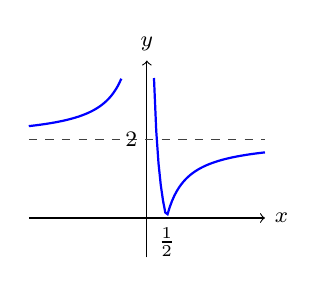
\begin{tikzpicture}[scale=0.5]
                      \draw [->] (-3,0) -- (3,0) node [right] {\footnotesize$x$};
                      \draw [->] (0,-1) -- (0,4) node [above] {\footnotesize$y$};

                      \draw [domain=-3:-0.65, samples=50, thick, blue] plot (\x, {abs((1/\x)-2)});
                      \draw [domain=0.18:3, samples=50, thick, blue] plot (\x, {abs((1/\x)-2)});

                      \draw [domain=-3:3, samples=10, darkgray, dashed] plot ({\x},2);

                      \node [left] at (0,2) {\footnotesize$2$};
                      \node [below] at (0.5,0) {\footnotesize$\frac{1}{2}$};
                  \end{tikzpicture}
            \item Gambarkan fungsi $f(x)=|4+|x-1||$
        \end{enumerate}
    \end{exampleblock}
\end{frame}

\end{document}